
\section{Related Work}
Our work lies within the field of video understanding using language, specifically targetted towards the visual question answering task. We use spatio-temporal scene graphs to generate our questions, and provide a suite of new evaluation metrics to measure compositional reasoning.

\noindent\textbf{Video Understanding}
Previous work pursues video understanding abilities through by creating data representations and using tasks that jointly reason over video and language. 
Videos have also been used to inform data structures and representations like graphs representing the social dynamics of movies and graphs \cite{vicol2018moviegraphs} representing the commonsense understanding of what likely occurred before and after a still image \cite{park2020visualcomet}. Studies on action recognition \cite{fernando2016discriminative, song2016multimodal}, temporal localization of actions \cite{anne2017localizing,gao2017tall}, and action sequence prediction \cite{nagarajan2020ego} match video content with language description of actions. Video captioning generates natural language descriptions of videos \cite{gan2017semantic, guadarrama2013youtube2text, venugopalan2015sequence}. Video Question Answering is another task that uses language to measure video understanding. Compared to current video understanding explorations, AGQA measures a wider variety of compositional spatio-temporal reasoning abilities. 

\noindent\textbf{Visual Question Answering}
Visual Question Answering is a task for checking visual reasoning skills by asking a model questions about visual input. A wide variety of benchmark datasets were created with images in the ImageQA task ~\cite{johnson2017clevr,hudson2019gqa,antol2015vqa,zellers2019recognition,goyal2017making,krishna2017visual,zhu2016visual7w,kim2020answering}. These benchmarks vary in input, from synthetic datasets~\cite{johnson2017clevr}, to cartoons~\cite{antol2015vqa}, to charts~\cite{kim2017deepstory}, to real-world images~\cite{hudson2019gqa,krishna2017visual,zhu2016visual7w,goyal2017making,zellers2019recognition,antol2015vqa}. They also vary in the type of questions asked, from descriptive 7W's (who, what, where, when, which, why, how)~\cite{zhu2016visual7w}, to commonsense reasoning~\cite{zellers2019recognition}, to compositional reasoning~\cite{johnson2017clevr,hudson2019gqa}, to spatial localization~\cite{zhu2016visual7w,krishna2017visual,hudson2019gqa}. These benchmarks facilitated the development of many models made to tackle these challenges by measuring their spatial reasoning abilities~\cite{lu2016hierarchical, vatashsky2020vqa, chen2020counterfactual}. However, ImageQA cannot measure temporal reasoning beyond guessing what might happen based on common sense \cite{zellers2019recognition}.

A growing interest in Visual Question Answering has also lead to the development of some VideoQA benchmarks~\cite{tapaswi2016movieqa,lei2018tvqa,jang2017tgif,kim2017deepstory,xu2017video,maharaj2017dataset,zeng2016leveraging,yu2019activitynet, yi2019clevrer}. Several of these prominent benchmarks rely on dialogue and plot summaries to reason over the contents of videos~\cite{lei2018tvqa,tapaswi2016movieqa,kim2017deepstory, zadeh2019social}. Models trained on these datasets have demonstrated a stronger dependence on the dialogue input than on the visual input, reducing these benchmarks' effectiveness at measuring visual spatio-temporal reasoning~\cite{tapaswi2016movieqa,lei2018tvqa}. Therefore, our project focuses pure video-only question answering benchmark. 

Some video-only question-answering benchmarks are synthetically generated \cite{yi2019clevrer, mun2017marioqa}. The granular control over what is synthetically generated allows for these benchmarks to measure concepts like causality and prediction \cite{yi2019clevrer}, or action sequences, counting, and the state of a virtual subject \cite{mun2017marioqa}. However, they use short video clips, work on a smaller set of objects and lack the diversity of visual features of real-world videos. Furthermore, they do not focus on human object interaction and activities as we do.

%\mgm{order this paragraph more like the intro}
Vision-only, real-world benchmarks exclusively ask questions that can be answered from a single frame of the video, questions that apply to the entire video with no temporal localization, or questions that ask "what happened before/after/while $<$action$>$?". They all, except~\cite{yu2019activitynet,xu2017video, zeng2016leveraging}, refer to videos of less than 10 seconds long.  Some have automatically generated questions from image descriptions~\cite{xu2017video,zeng2016leveraging}, some let human annotators choose from drop down menus~\cite{jang2017tgif}, and others ask humans annotators to create questions~\cite{yu2019activitynet,tapaswi2016movieqa,jang2017tgif,lei2018tvqa}. The largest dataset with solely human generated questions is~\cite{lei2018tvqa} with 152.5K question answer pairs, and the largest dataset with solely automatically generated questions is~\cite{maharaj2017dataset} with 349K question answer pairs. Our dataset is purely vision based, works on videos of 2-195 seconds long, and evaluates complex and multi-step temporal reasoning. \mgm{Very much a laundry list of just x y z. Maybe will do They are x, we are y. They are a, we are b structure? Otherwise take out less interesting stuff}


\noindent\textbf{Scene graphs.}
Scene graphs are a symbolic representation of an image~\cite{krishna2017visual}. The graph consists of nodes representing the objects in the image and edges representing relationships between those objects. For each object node there are associated attributes. For example, an image with a man wearing white shorts would have an object node for "shorts" with "white" as an attribute and an object node for "man". These object nodes would be connected by an edge representing the relationship "wearing". Creating this symbolic representation of an image reduces it to its semantic parts. Using this representation has improved performance on many visual tasks such as Visual Question Answering~\cite{johnson2017inferring}, relationship modeling~\cite{krishna2018referring}, image captioning and evaluation ~\cite{anderson2016spice}, image generation~\cite{johnson2018image,ashual2019specifying}, and image retrieval ~\cite{ashual2019specifying,johnson2015image}. Of particular interest to our project is how scene graphs were used by GQA for visual question answer generation~\cite{hudson2019gqa}.

Inspired by Visual Genome's scene graphs,~\cite{ji2020action} annotated spatio-temporal scene graphs to create Action Genome. Spatio-temporal scene graphs consist of nodes representing objects and edges representing relationships between them. Each of these objects are associated with a specific frame in the video. The resulting effect is that a subject's relationships with the objects changes over time. Unlike GQA, we use spatio-temporal scene graphs for question answer generation over videos. 

\noindent\textbf{Compositional reasoning.}
As questions become more complex, they often require multiple reasoning steps in order to find the answer. For example, the question "Was the person running or sitting for longer?" first requires finding the start and end of when the person was running and sitting, subtracting the start from the end, then comparing the lengths of each action's occurrence. A constrained set of logical steps (e.g. action localization, subtraction, comparison, etc.) can be used as building blocks that are reordered to respond to a wide variety of different questions. This multi-step reasoning is called compositional reasoning because the overall understanding is composed of a series of smaller reasoning steps. Humans are able to learn quickly by generalizing new information in existing contexts~\cite{tani2014self,schulz2016probing}. Improving a model's ability to generalize will allow it to more quickly learn new domains, categories, and logical rules~\cite{lake2018generalization,vatashsky2020vqa}. 

Some metrics for evaluating compositionality in language corpuses have been defined \cite{keysers2019measuring,lake2018generalization}, and some ImageQA benchmarks use compositional reasoning extensively~\cite{johnson2017clevr,hudson2019gqa}. but beyond the synthetic dataset CLEVRER~\cite{yi2019clevrer}, no VideoQA datasets go beyond three steps of compositional reasoning in a question. 
%Although these logical building block steps have been defined for ImageQA~\cite{cheng2015break}, there are no compositional reasoning steps defined for temporal reasoning. \mgm{take this out? Don't define them in this paper.}
Current models have struggled with multi-step reasoning, motivating a benchmark like ours that specifically explores compositional reasoning~\cite{fan2019heterogeneous}.

%Compositional questions have been used by ImageQA benchmarks to rigorously test models. Compositional questions tend to be longer, more complex, and use a wider variety of vocabulary~\cite{johnson2017clevr,hudson2019gqa,lake2018generalization}. Furthermore, they can better test a model's reasoning ability both by requiring multiple steps of reasoning to answer the questions and by allowing for datasets to test generalization to novel compositions~\cite{lake2018generalization}. 
%For example, on the CLEVR dataset, the training questions could include the phrases "right of cube" and "behind sphere", but not "right of sphere" as a combination. Testing on this novel combination "right of sphere" in the test set tests a model's ability to generalize to new concepts~\cite{lake2018generalization,johnson2017clevr}. 

Many questions relevant to reasoning over videos require multi-step reasoning. A simple example covered by current datasets involves first localizing in time, then reasoning about that specific time. For example, this question from~\cite{jang2017tgif}, "What does the model do after
lower coat?", requires finding when the model lowers her coat, then determining her activity after that. Another way to reason compositionally \mgm{is this a word?} is to refer to subjects indirectly, as the ImageQA benchmark~\cite{hudson2019gqa} does with "What color is the food on the red object to the left of the girl?". We use both temporal localization and indirect references to increase question compositionality, and we implement several metrics to measure different compositional reasoning abilities than existing Visual Question Answering benchmarks.



\rak{this paragraph feels better suited for related work. I moved it from the introduction.}
Existing question-answering benchmarks are limited in the diversity of their questions. Since most benchmarks are image-based, they only test a model's reasoning over spatial relationships~\cite{johnson2017clevr,hudson2019gqa,antol2015vqa,goyal2017making,krishna2017visual,zhu2016visual7w}, object attributes~\cite{johnson2017clevr,hudson2019gqa, antol2015vqa,goyal2017making,krishna2017visual}, and common sense understanding~\cite{zellers2019recognition,antol2015vqa,krishna2017visual}. These benchmarks are unable to test reasoning over temporal relationships or activities beyond guessing based on common sense knowledge \cite{zellers2019recognition}. All questions asked by VideoQA benchmarks on non-synthetic videos that do not include extra textual information like dialogue limited temporal localization. Temporal localization refers to using the phrase "before/after/while $<$action$>$" to localize a relevant time in the video over which to reason. Questions in these benchmarks 1) can be answered from a single frame of the video, 2) apply to the entire video with no temporal localization, or 3) ask "what happened before/after/while $<$action$>$?"~\cite{jang2017tgif,xu2017video, maharaj2017dataset, zeng2016leveraging, yu2019activitynet}. Of the questions that apply to the entire video, some spatio-temporal topics are measured like counting and object and action recognition.


 
\rak{More text I moved over from the introduction.}
Models should also be able to perform more complex temporal localization, follow the changing state of objects over time, sequence actions, and understand the concepts of action length, first, and last~\cite{lake2018generalization,vatashsky2020vqa}.

Beyond measuring limited spatio-temporal reasoning, no existing benchmarks we know of measures a model's ability to generalize to new information. CLEVRER looks at compositional questions, but does not create metrics designed for measuring compositional reasoning \cite{yi2019clevrer}. Measuring models on compositional questions measures their ability to generalize from simple building blocks of information to more complex combinations. We adapt strategies from the constrained evaluation of the SCAN dataset \cite{lake2018generalization} to measure models' abilities to generalize to novel combinations of ideas, to adding temporal localizations and indirectly referencing ideas, to videos of longer lengths, and to more complex question structures.

\begin{figure*}[t]
    \centering
    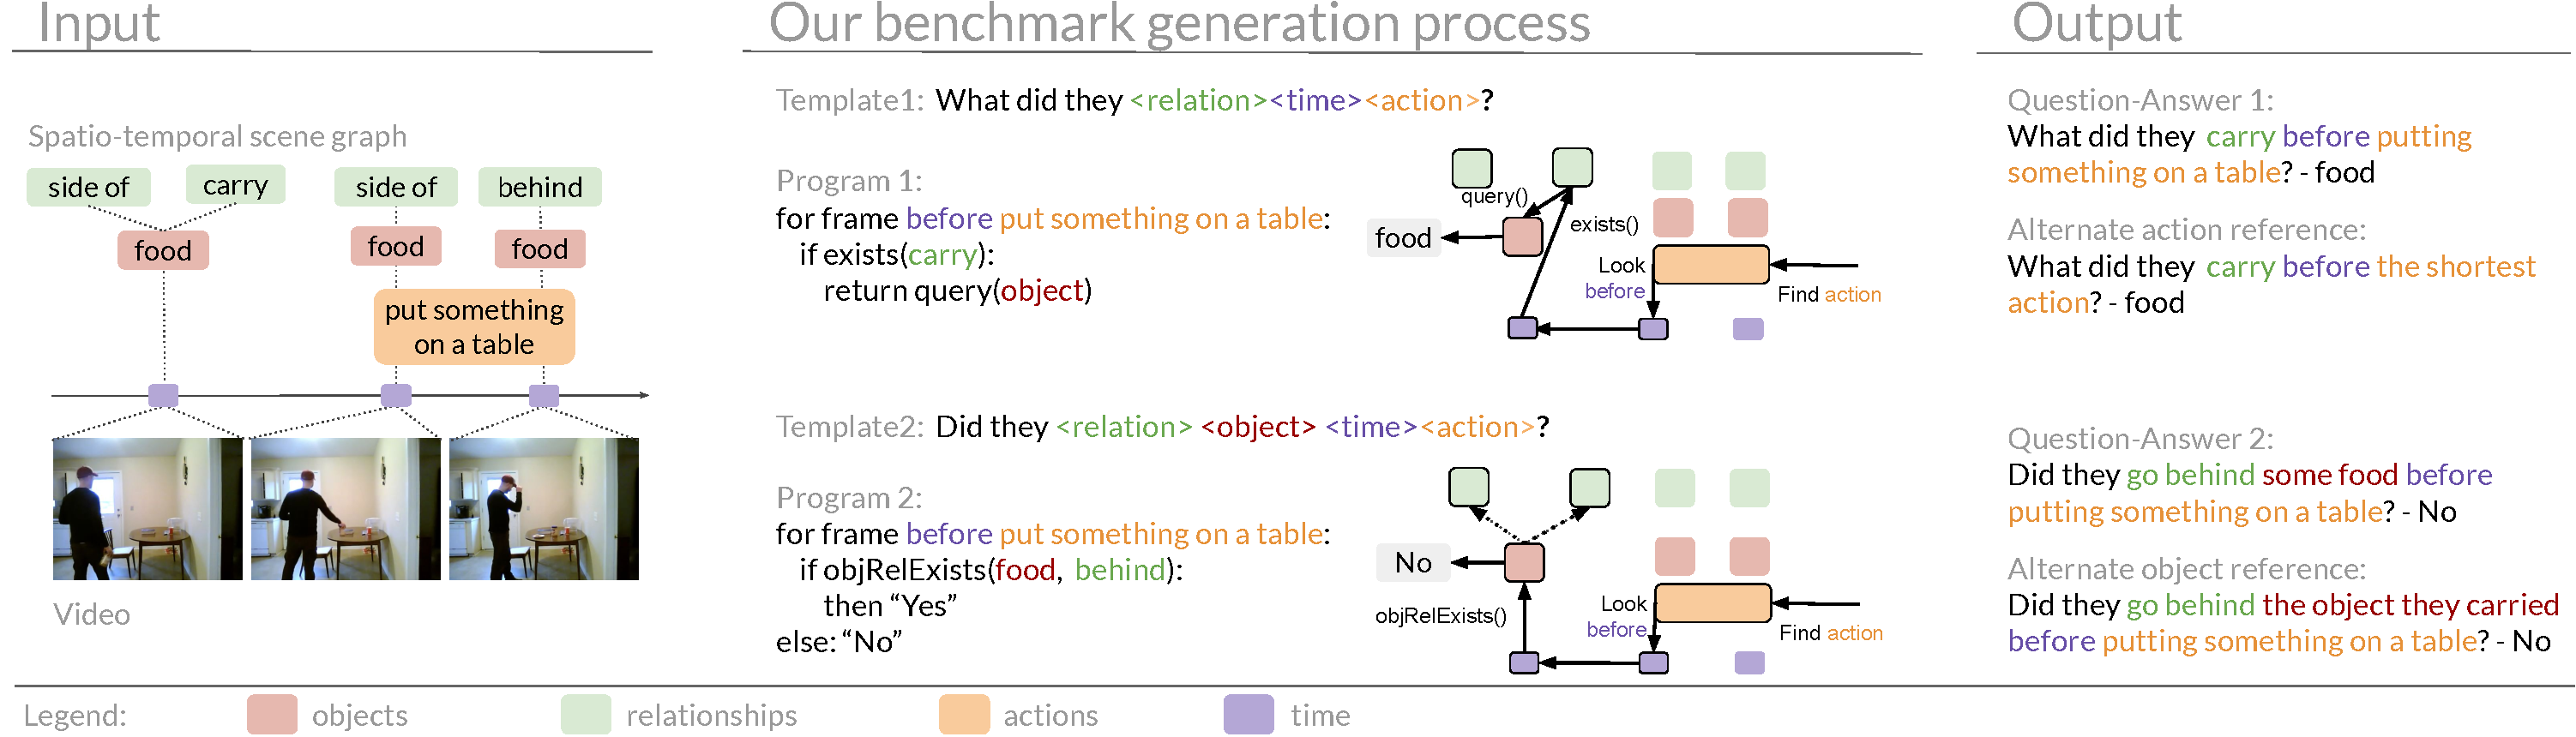
\includegraphics[width=0.95\linewidth]{figures/system.pdf}
    \caption{\textbf{Input:} To generate questions, we first ground the video in the \object{object}, \relationship{relation}, \action{action}, and \temporal{frame} level visual primitives by augmenting Action Genome's spatio-temporal scene graphs~\cite{ji2020action} and Charades' action annotations~\cite{sigurdsson2016hollywood}.  \mgm{add color}. \textbf{Our benchmark generation process:} we built a series templates with $<$tags$>$ that can be filled in with the associated primitive to generate a natural language question. Each template is also associated with a unique program that reasons over the spatio-temporal scene graph to automatically generate the answer to the question. \textbf{Output: } We create a dataset of question-answer pairs. Question diversity is increased by referencing primitives by their qualities (e.g. 'shortest action') or interactions (e.g. 'the object they carried').}
    \label{fig:system}
\end{figure*}